\documentclass[../Main/main.tex]{subfiles}

\begin{document}
\graphicspath{{../numerical results/figs/}}
		\chapter{Numerical Results}
		In this chapter we do several numerical experiments with the algorithms covered in this thesis. And briefly discuss the code used to do the experiments.
		\section{Computer Code}
		Most of the code used in this thesis can be found on \href{https://github.com/trulsmoholt/masterthesis}{https://github.com/trulsmoholt/masterthesis}, and is written in python and numpy. It is primarily intended for educational purposes and for comparing convergence rates of different spatial approximation techniques. An example of a very simple use case can be seen in \ref{l:1} \\
		\begin{minipage}{\linewidth}
			\begin{lstlisting}[language=Python,caption=Solving simple Poisson equation.,label=l:1]

from discretization.mesh import Mesh
from discretization.FVML import compute_matrix,compute_vector
import numpy as np
import math

#Function to perturb mesh from unit square. Takes a 2d numpy vector and returns a 2d numpy vector. This particular choice makes a paralellogram mesh.
perturbation=lambda p: np.array([p[0],0.5*p[0]+p[1]])

#Number of grid points in x and y direction
nx=ny=10

mesh = Mesh(nx,ny,perturbation,ghostboundary=True)
source = lambda x,y:math.sin(y)*math.cos(x)
boundary_condition = lambda x,y:0
tensor = np.eye(2)
permeability = np.ones((mesh.num_unknowns,mesh.num_unknowns))

A = np.zeros((mesh.num_unknowns,mesh.num_unknowns))#stiffness matrix
f = np.zeros(mesh.num_unknowns)#load vector

compute_matrix(mesh,A,tensor,permeability)
compute_vector(mesh,f,source,boundary_condition)

u = np.linalg.solve(A,f)
mesh.plot_vector(u)
			\end{lstlisting}
		\end{minipage}
		
		The code is centred around the mesh class, which contains information about how the domain is discretized into quadrilaterals and its properties. This class also contains public functions to make plots of different kinds and compute errors. The spatial numerical methods implemented are: TPFA, MPFA-L, MPFA-O and linear Lagrange finite elements. They all have the same call signature, as in \ref{l:1} line 22 and 23. The control volume methods also has the option of taking a matrix to store the flux stencils. One can use sparse matrices instead of dense numpy matrices in \ref{l:1}, as long as the indexing signature is the same as in numpy, for example scipy has a compatible sparse matrix library.
		\par
		The code also has implementations of mass matrix and the gravitation term. Also included in the github are an example of how to solve Richards' equation using L-scheme linearization and backward Euler, see \ref{l:2} for some of the code.
		\begin{minipage}{1.1\linewidth}
			\centering
\begin{lstlisting}[language=Python,caption=Linearization and time stepping of Richards' equation.,label=l:2]
u_l = u.copy() #linearization/L-scheme iterate
u_t = u.copy() #timestep iterate
F = u.copy() #source vector
A = np.zeros((mesh.num_unknowns,mesh.num_unknowns)) #stiffness matrix
B = mass_matrix(mesh)

#time iteration
for t in time_partition[1:]:
	#empty source vector
	F.fill(0)
	#compute source vector
	compute_vector(mesh,F,lambda x,y: f(x,y,t),lambda x,y:u_exact(x,y,t))
	#L-scheme iteration
	while True:
		#compute the heterogeneous hydraulic conductivity, kappa
		conductivity = kappa(np.reshape(u_l, (mesh.cell_centers.shape[0],mesh.cell_centers.shape[1]),order='F'))
		A.fill(0)#empty the stiffness matrix
		compute_matrix(mesh, A, K,conductivity)#compute stiffnes matrix
		lhs = L*B+tau*A
		rhs = L*B@u_l + B@theta(u_t) - B@theta(u_l) + tau*F
		u = np.linalg.solve(lhs,rhs)
		#check if L-scheme linearization has acceptable error
		if np.linalg.norm(u-u_l)<=TOL+TOL*np.linalg.norm(u_l):
			#quit linearization and do another time step
			break
		else:
			#update linearization iterate
			u_l = u
	#update time step iterate		
	u_t = u
	#update linearization iterate
	u_l = u
\end{lstlisting}		\end{minipage}
		
		\
		\section{Elliptic Equation}
		\label{sec:elliptic_numerical}
		The convergence tests in this section are similar to some of the tests done in chapter three of \cite{https://doi.org/10.1002/num.20320}. We consider the elliptic model problem \eqref{eq:poisson}, find $u\in H^1_0(\Omega)$ such that
		\begin{equation} \label{eq:model}
			\begin{split}
				\nabla \cdot \bm{q} &= f \\
				\bm{q} &= -\bm{K}\nabla u.
			\end{split}
		\end{equation}
		We set the solution
		\begin{equation}\label{eq:pressure_solution_model}
			u = cosh(\pi x)cos(\pi y)
		\end{equation} 
		And set $\bm{K}$ to be the identity matrix. 
		As in \cite{https://doi.org/10.1002/num.20320} page 1340 we define the normalized discrete $L_2$ norms:
		\begin{equation}
			\left \| u - u_h \right \|_{0,h} =  \left (  \frac{1}{V}\sum_i V_i(u_{h,i}-u_i)^2\right )^{\frac{1}{2}}
		\end{equation}
		\begin{equation}\label{eq:normal_flow_density}
			\left \| q - q_h \right \|_{0,h} =  \left (  \frac{1}{Q}\sum_a Q_a(q_{h,a}-q_a)^2\right )^{\frac{1}{2}},
		\end{equation}
		where $q_a := -\bm{\hat{n}} \cdot \bm{q}$ is the normal flow density over edge $a$, with $\bm{\hat{n}}$ being unit normal to the edge and $\bm q$ evaluated at the midpoint of the edge. $q_{h,a}$ is the discrete flux over $a$ defined similarly with $\bm{q}_h$ being the discrete normal flow density, for a finite volume method this would be the flux across some edge divided by the edge length. 
		For the finite element method, we use the MPFA-L flux stencil to recover the flux in the experiments where it is present.
		 Let $u_{h,i}$ denote the discrete potential at cell $i$, and $u_i$ is the potential evaluated at cell $i$. For the finite element method, this would be the function value at the grid points/nodes. $Q_a$ is the volume associated with edge $a$, i.e., the sum of the two volumes sharing edge $a$. $V = \sum_{i} V_i$ and $Q = \sum_{a} Q_a$.
		\par 
		In the figures (5.12-5.15) in this section we see convergence rates in the $\left \| \cdot \right \|_{0,h}$ norm for different spatial numerical methods. The y-axis is the $log_2$ of the error and the x-axis is $log_2n$, where $n$ is the number of points in x and y direction, and thus proportional with the inverse of the mesh diameter. The slope of the graph in the plots are the convergence rate.
		\par
		In figures \ref{fig:mesh_uniform_potential} and \ref{fig:mesh_uniform_potential} we see that all the methods converge with the same quadratic rate. This fits well with the fact that all the methods covered in this thesis are equivalent to the TPFA method for uniform grids.
		\par
		In figures \ref{fig:mesh_trapezoidal}, \ref{fig:mesh_trapezoidal_potential} and \ref{fig:mesh_trapezoidal_flow} we observe that the TPFA method does not converge for parallelogram mesh. This makes sense as the grid is not K-orthogonal. The others methods still have quadratic convergence for potential and flow density.
		\par
		In figures \ref{fig:mesh_perturbed}, \ref{fig:mesh_perturbed_potential} and \ref{fig:mesh_perturbed_flow} the MPFA-L, MPFA-O and FEM still converges quadratically for the potential on a rough grid, where every grid point is perturbed randomly by a factor proportional to the gird diameter. For the normal flow density however, the convergence rate drops to about one.
		\par 
		In figure \ref{fig:mesh_perturbed_1d2} we introduce grids with aspect ratio, that is grids with more points in the y direction.
		In figure \ref{fig:mesh_perturbed_potential_1d10} we observe that MPFA-L, MPFA-O and FEM has a convergence rates for the potential of about 1.5 for the grid with aspect ratio 0.1. In figure \ref{fig:mesh_perturbed_potential_1d100} we see that the MPFA-O method fail to converge for the grid with aspect ratio 0.01. Thus the MPFA-L method wins this round of numerical experiments.
		\begin{figure}[h]
			\centering
			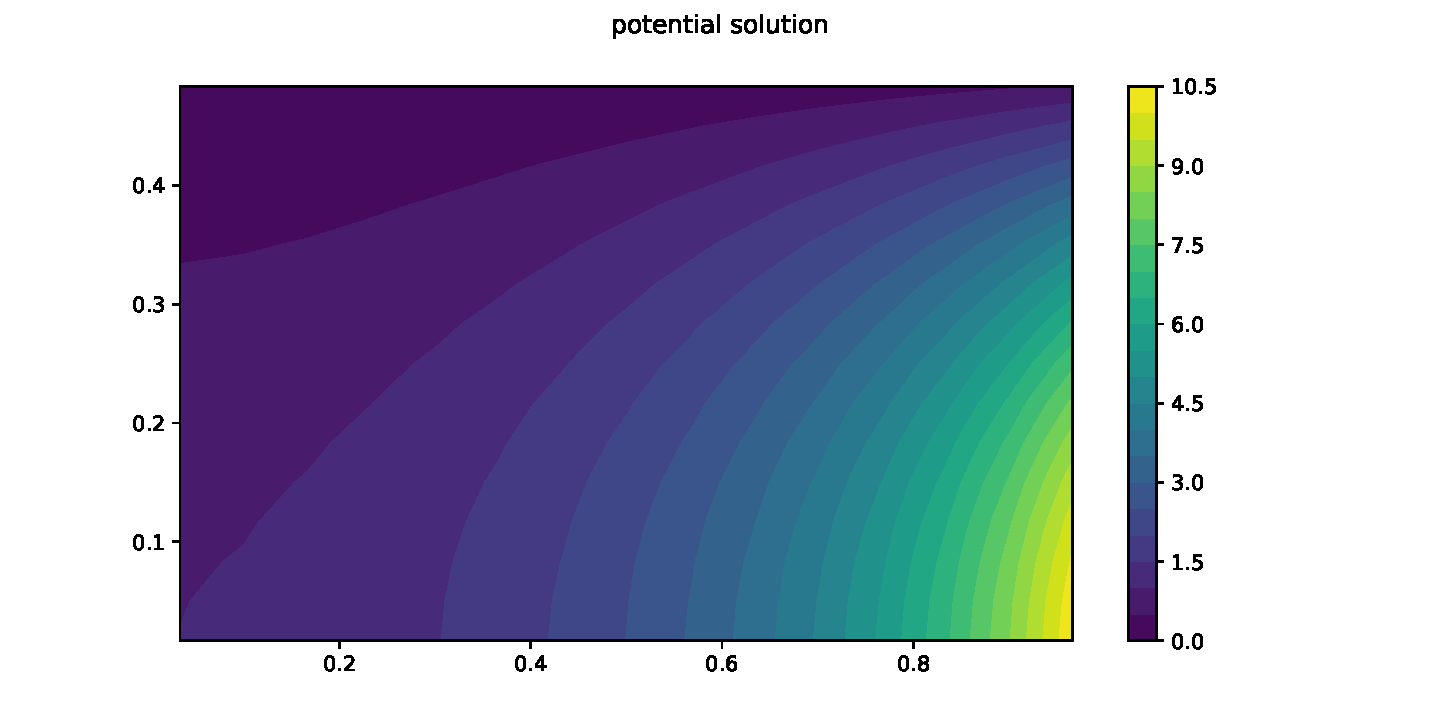
\includegraphics[width=1\textwidth]{Potential.pdf}
			\caption{The solution \eqref{eq:pressure_solution_model} on half the unit square }
			\label{fig:solution}
		\end{figure}
		\newpage
		\begin{figure}[H]
			\centering
			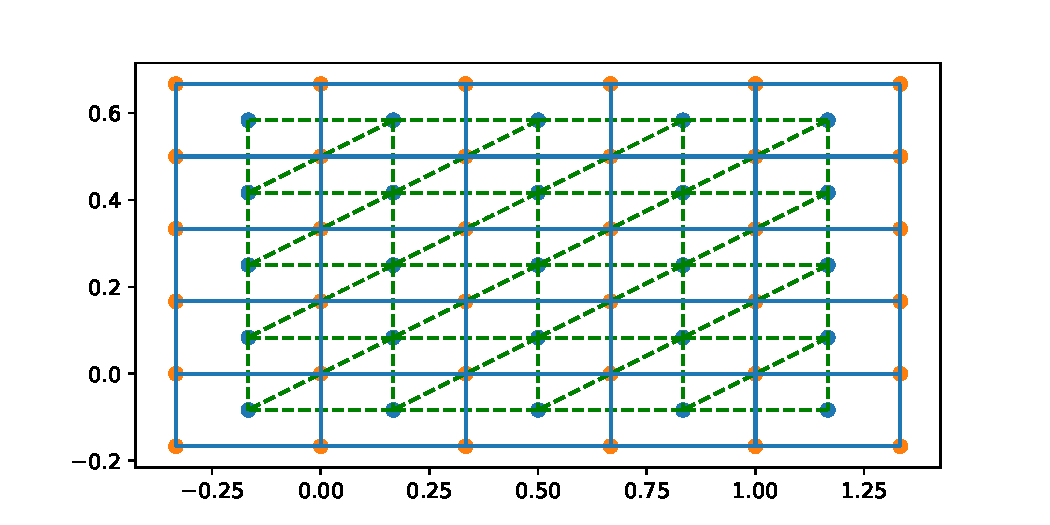
\includegraphics[width=1\textwidth]{orthognal_mesh.pdf}
			\caption{Unifrom rectangular mesh on half the unit square. The triangles are used for the finite element solution and are spanned between the nodes of the cell centers of the finite volume methods. The ghost cell boundary is included, so this mesh has nine degrees of freedom, i.e., the interior cells.}
			\label{fig:mesh_uniform}
		\end{figure}
		\begin{figure}[H]
					\advance\leftskip-1cm
			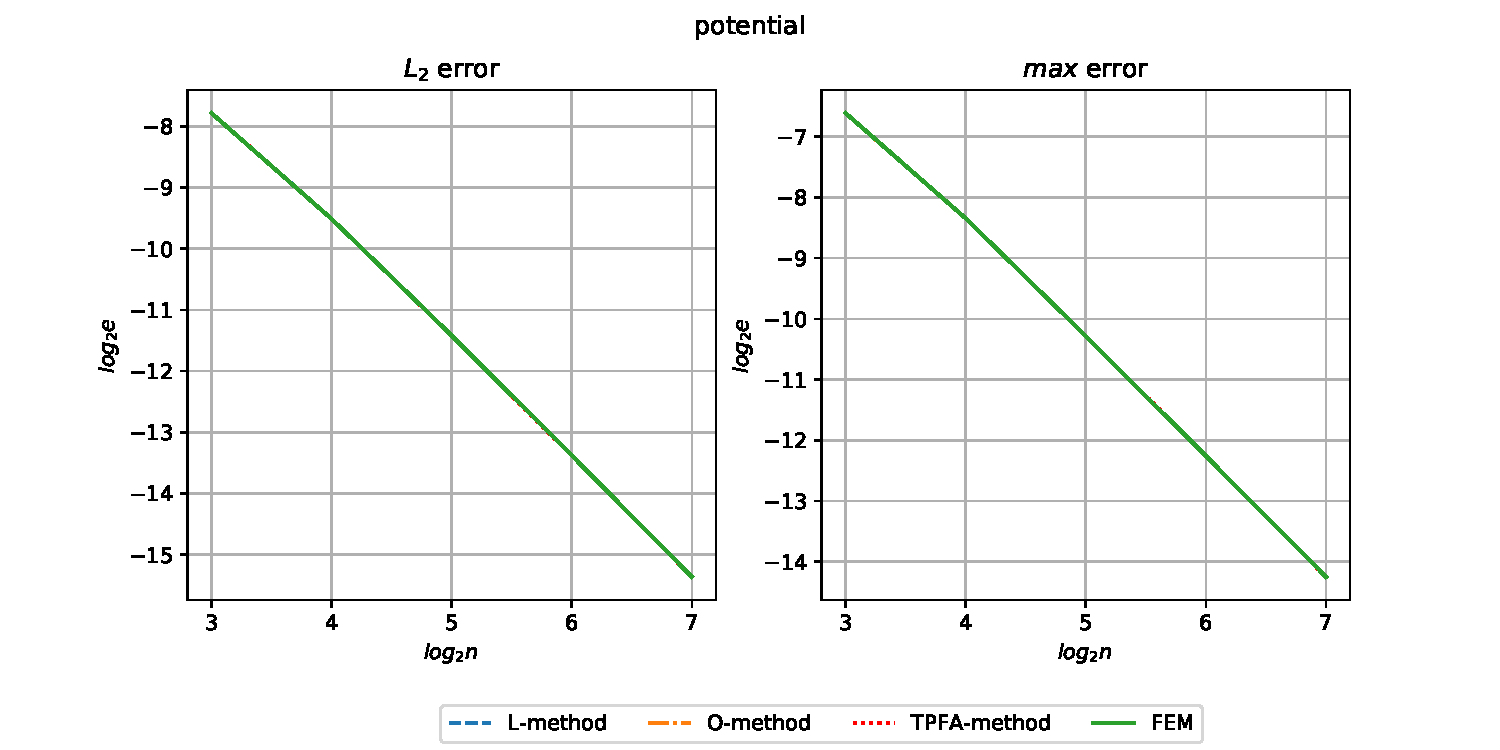
\includegraphics[width=1.2\textwidth]{pressure_quadratic.pdf}
			\caption{Potential error on refinements of the uniform rectangular mesh \ref{fig:mesh_uniform}. The convergence is the same for all the schemes.}
			\label{fig:mesh_uniform_potential}
		\end{figure}
		\begin{figure}[H]
			
			\advance\leftskip-1cm
			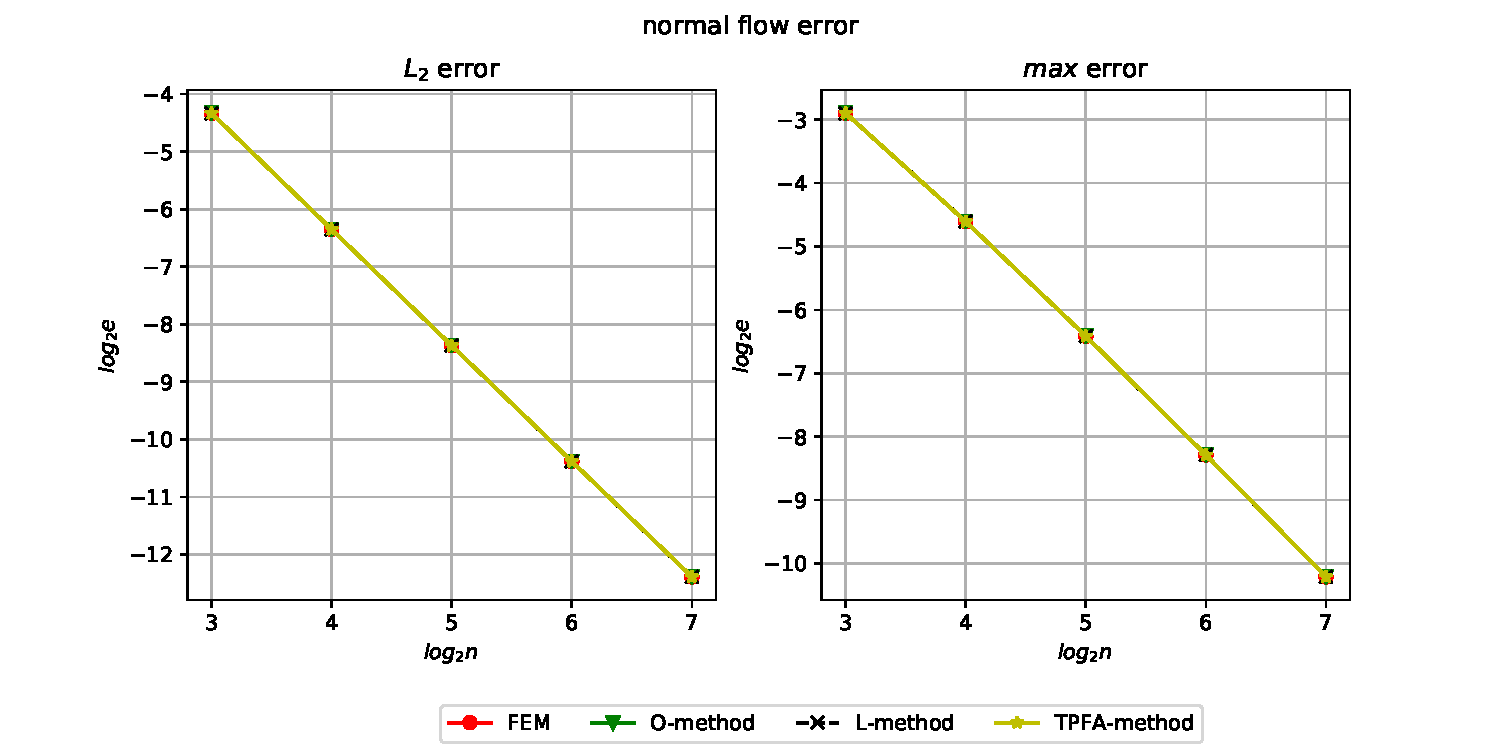
\includegraphics[width=1.2\textwidth]{flow_quadratic.pdf}
			\caption{Normal flow density error on refinements of the uniform rectangular mesh \ref{fig:mesh_uniform}. The convergence is the same for all the schemes.}
			\label{fig:mesh_uniform_flow}
		\end{figure}

		\begin{figure}[H]
			\centering
			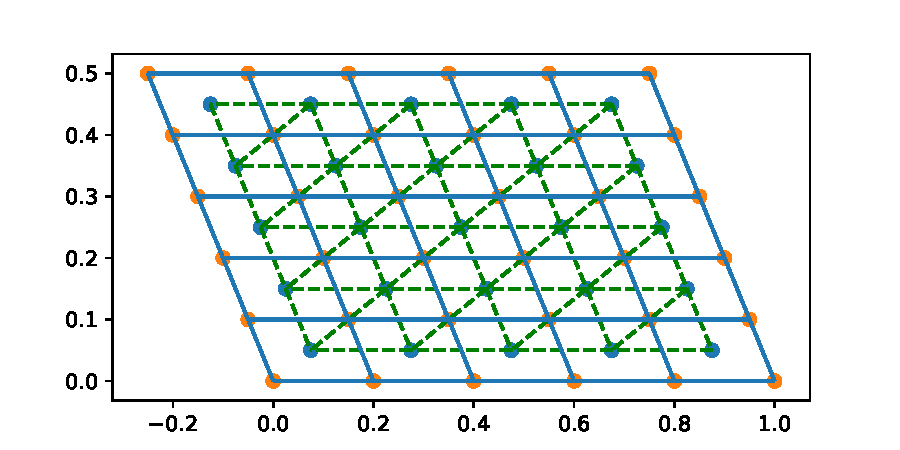
\includegraphics[width=1\textwidth]{mesh_trapezoidal.pdf}
			\caption{Trapezoidal mesh, now every point is transformed by $(x,y)  \mapsto (x-0.5y,y)$}
			\label{fig:mesh_trapezoidal}
		\end{figure}
	
	\begin{figure}[H]
		\advance\leftskip-1cm
		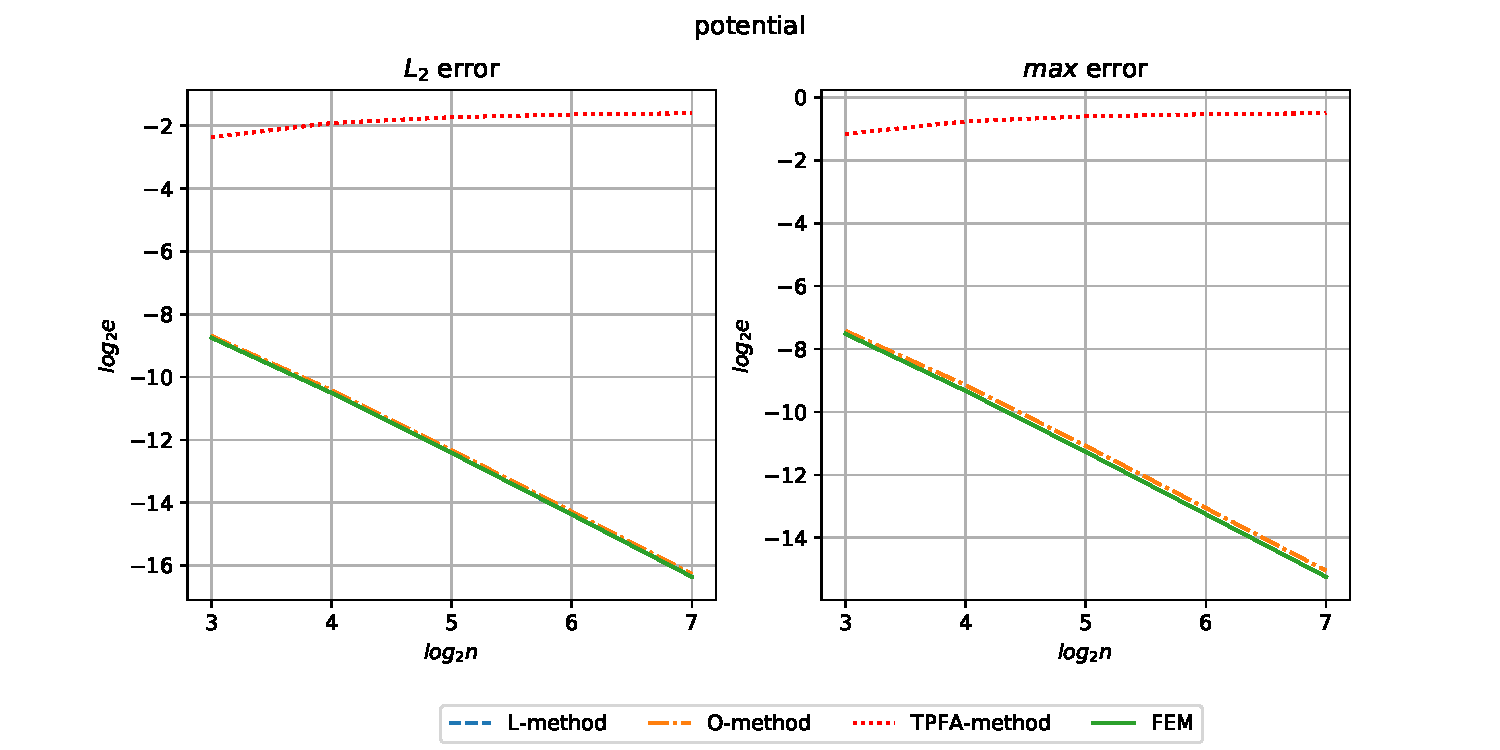
\includegraphics[width=1.2\textwidth]{pressure_trapezoidal_1d1.pdf}
		\caption{Pressure error on refinements of the mesh \ref{fig:mesh_trapezoidal}}
		\label{fig:mesh_trapezoidal_potential}
	\end{figure}
	\begin{figure}[H]
		\advance\leftskip-1cm
		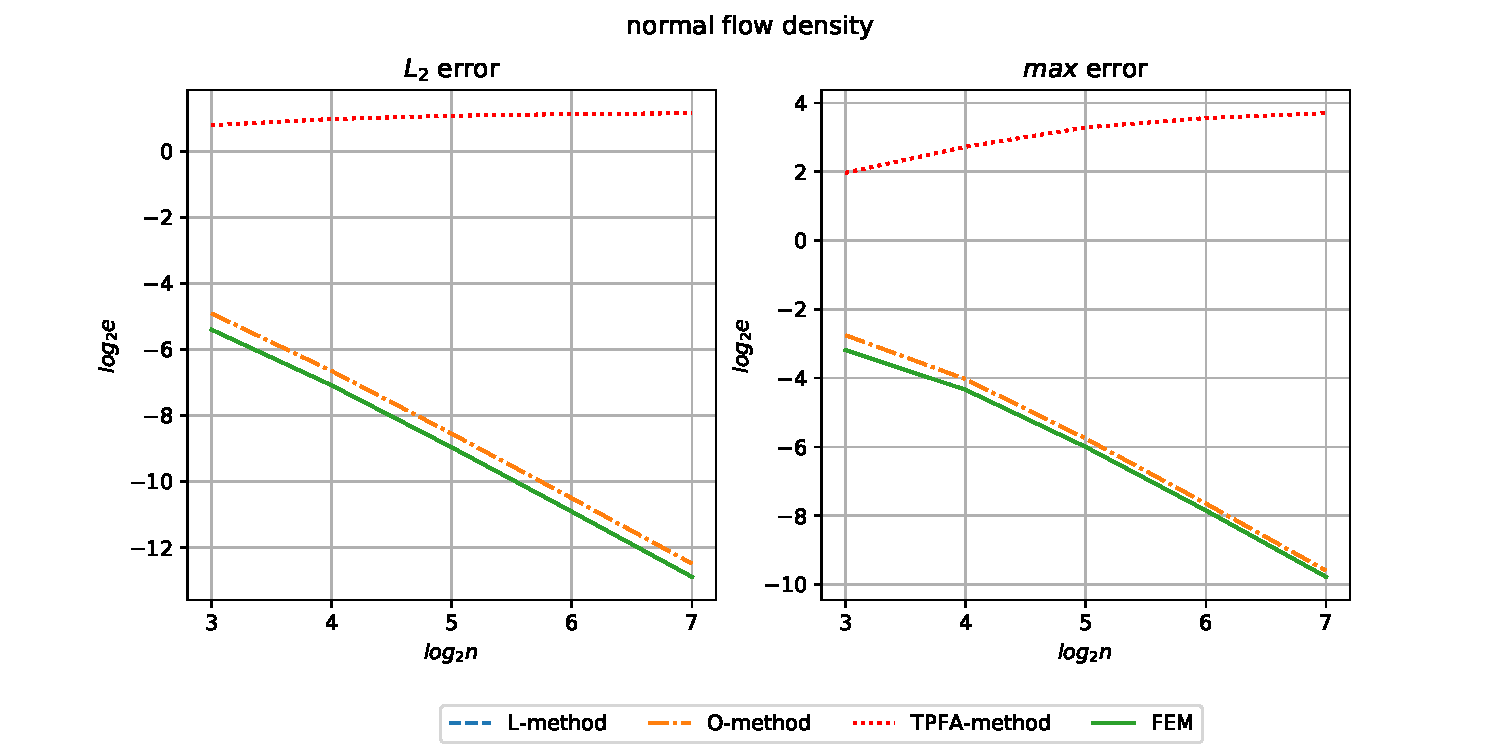
\includegraphics[width=1.2\textwidth]{flow_trapezoidal_1d1.pdf}
		\caption{Normal flow density error on refinements of the mesh \ref{fig:mesh_trapezoidal}}
		\label{fig:mesh_trapezoidal_flow}
	\end{figure}
	
		\begin{figure}[H]
			\centering
			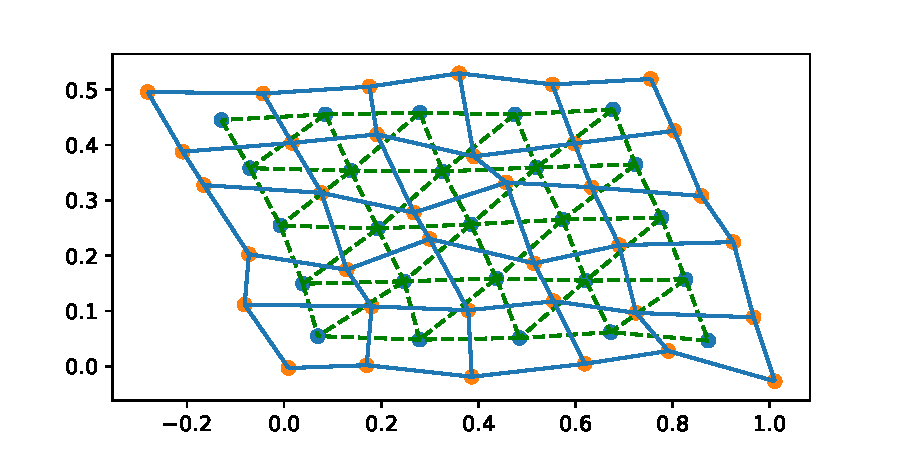
\includegraphics[width=0.9\textwidth]{mesh_perturbed.pdf}
			\caption{Perturbed mesh, every point in the mesh is perturbed by a random number which is $O(\frac{h}{5})$, in both x and y direction.}
			\label{fig:mesh_perturbed}
		\end{figure}
		\begin{figure}[H]
		\advance\leftskip-1cm
			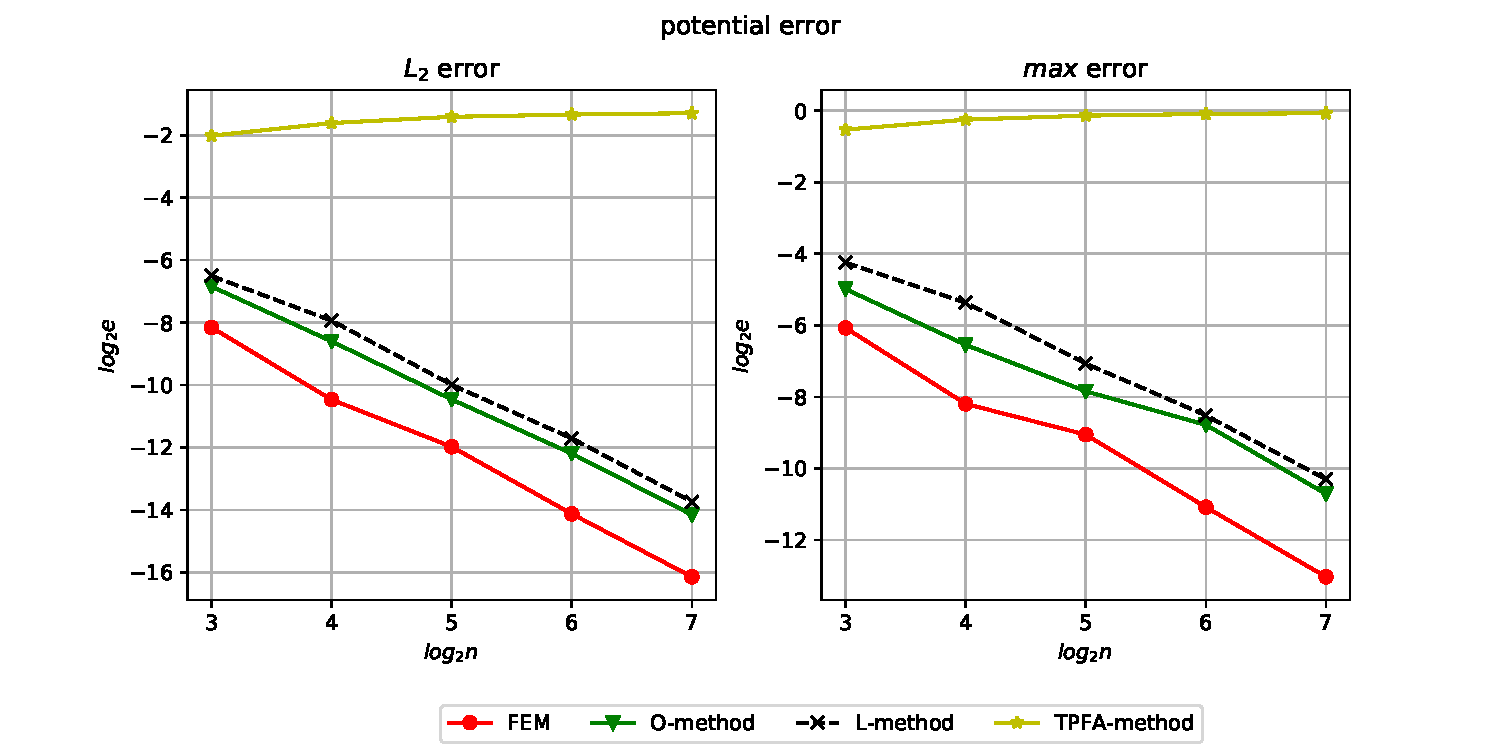
\includegraphics[width=1.2\textwidth]{pressure_perturbed_1d1.pdf}
			\caption{The pressure error of perturbed mesh.}
			\label{fig:mesh_perturbed_potential}
		\end{figure}
		\begin{figure}[H]
		\advance\leftskip-1cm
			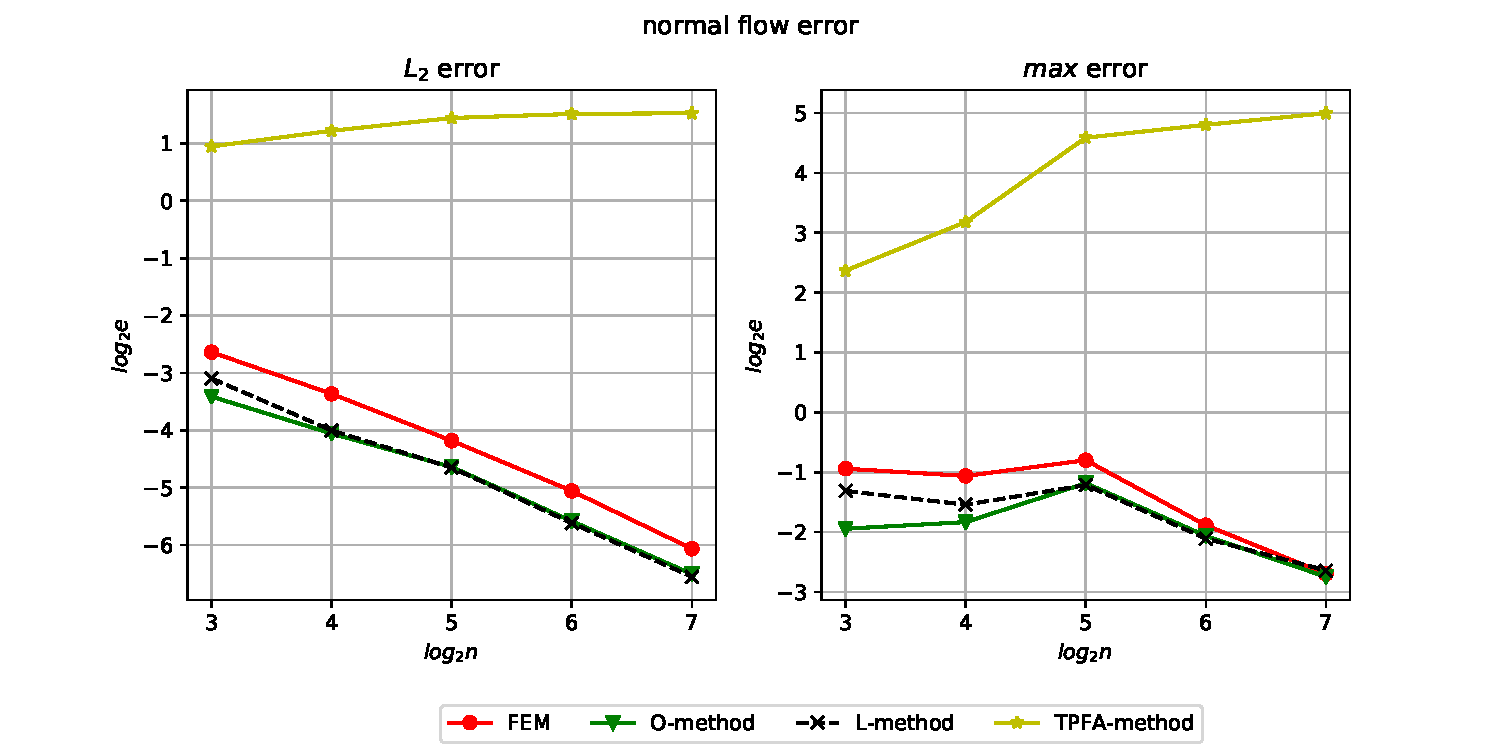
\includegraphics[width=1.2\textwidth]{flow_perturbed_1d1.pdf}
			\caption{The normal flow density error of perturbed mesh}
			\label{fig:mesh_perturbed_flow}
		\end{figure}
		\begin{figure}[H]
			\centering
			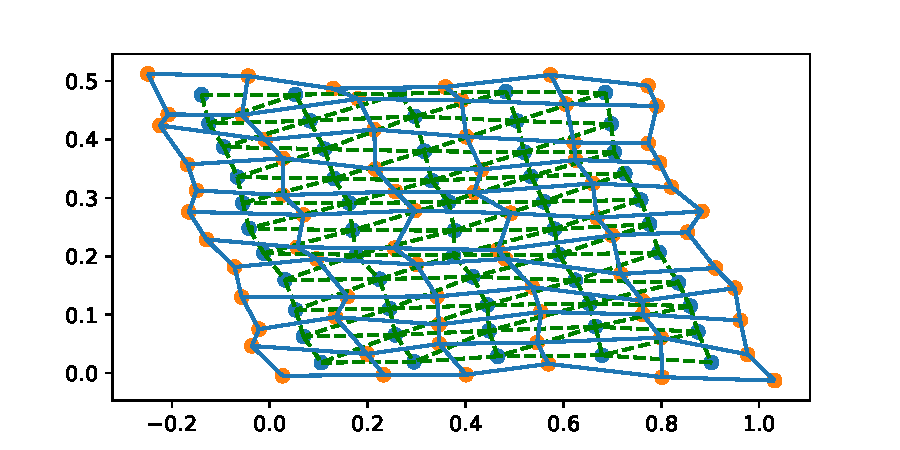
\includegraphics[width=1\textwidth]{mesh_perturbed_1d2.pdf}
			\caption{Perturbed mesh with aspect ratio 0.5, there are half as many points in the x-direction as in the y-direction.}
			\label{fig:mesh_perturbed_1d2}
		\end{figure}
		\begin{figure}[H]
		\advance\leftskip-1cm
			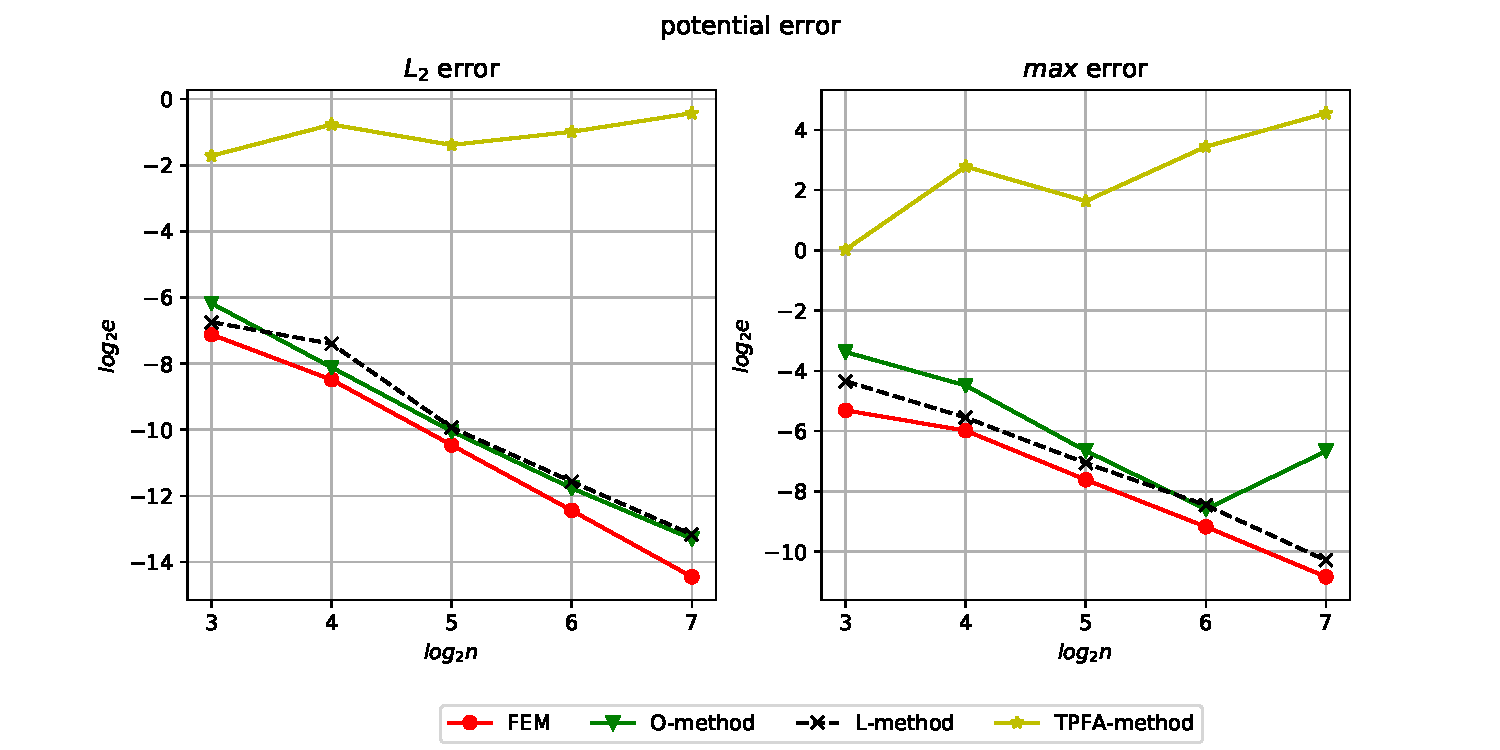
\includegraphics[width=1.2\textwidth]{pressure_perturbed_1d10.pdf}
			\caption{The pressure error of perturbed mesh with aspect ratio 0.1.}
			\label{fig:mesh_perturbed_potential_1d10}
		\end{figure}
			\begin{figure}[H]
			\advance\leftskip-1cm
			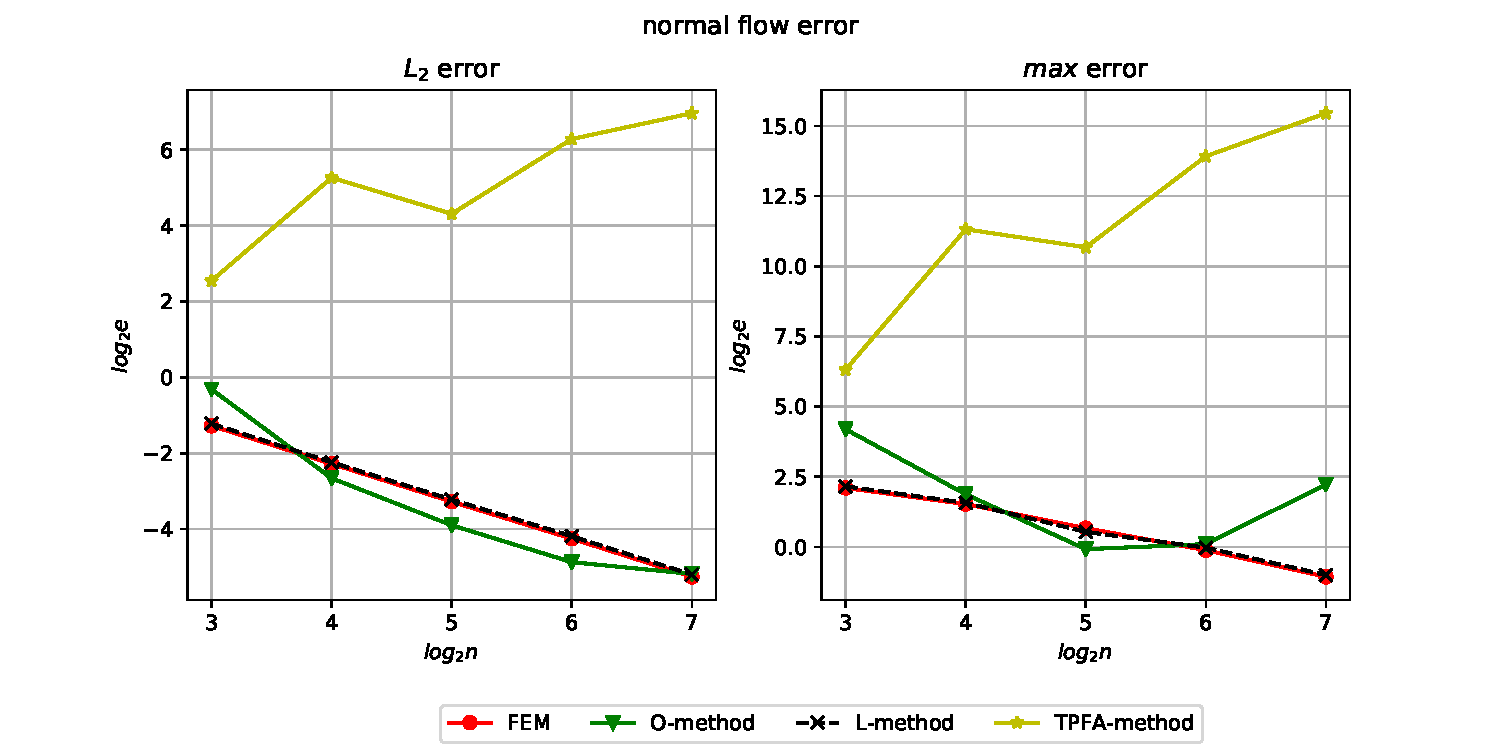
\includegraphics[width=1.2\textwidth]{flow_perturbed_1d10.pdf}
			\caption{The normal flow density error of perturbed mesh with aspect ratio 0.1.}
			\label{fig:mesh_perturbed_flow_1d10}
		\end{figure}
		\begin{figure}[H]
			\advance\leftskip-1cm
			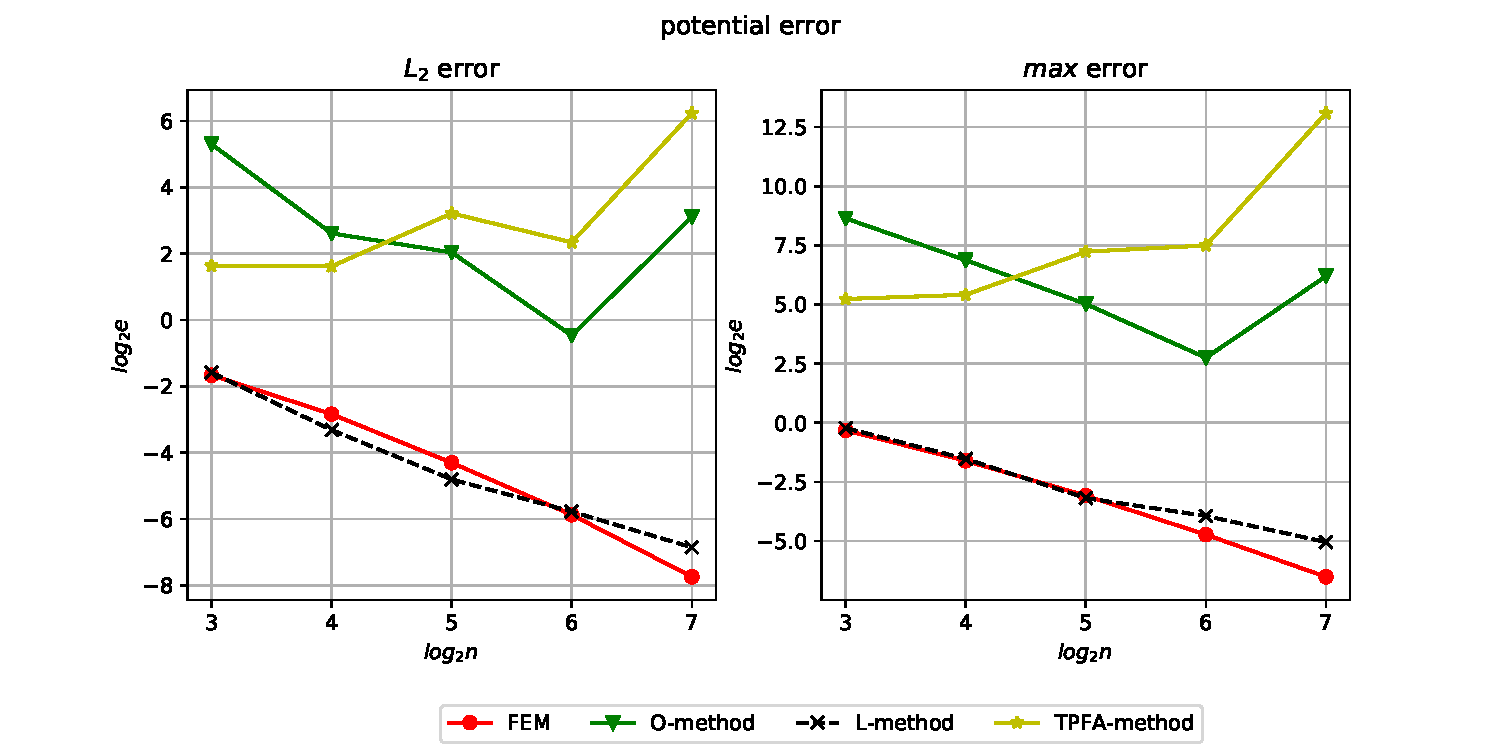
\includegraphics[width=1.2\textwidth]{pressure_perturbed_1d100.pdf}
			\caption{The pressure error of perturbed mesh with aspect ratio 0.01.}
			\label{fig:mesh_perturbed_potential_1d100}
		\end{figure}
		\begin{figure}[H]
			\advance\leftskip-1cm
			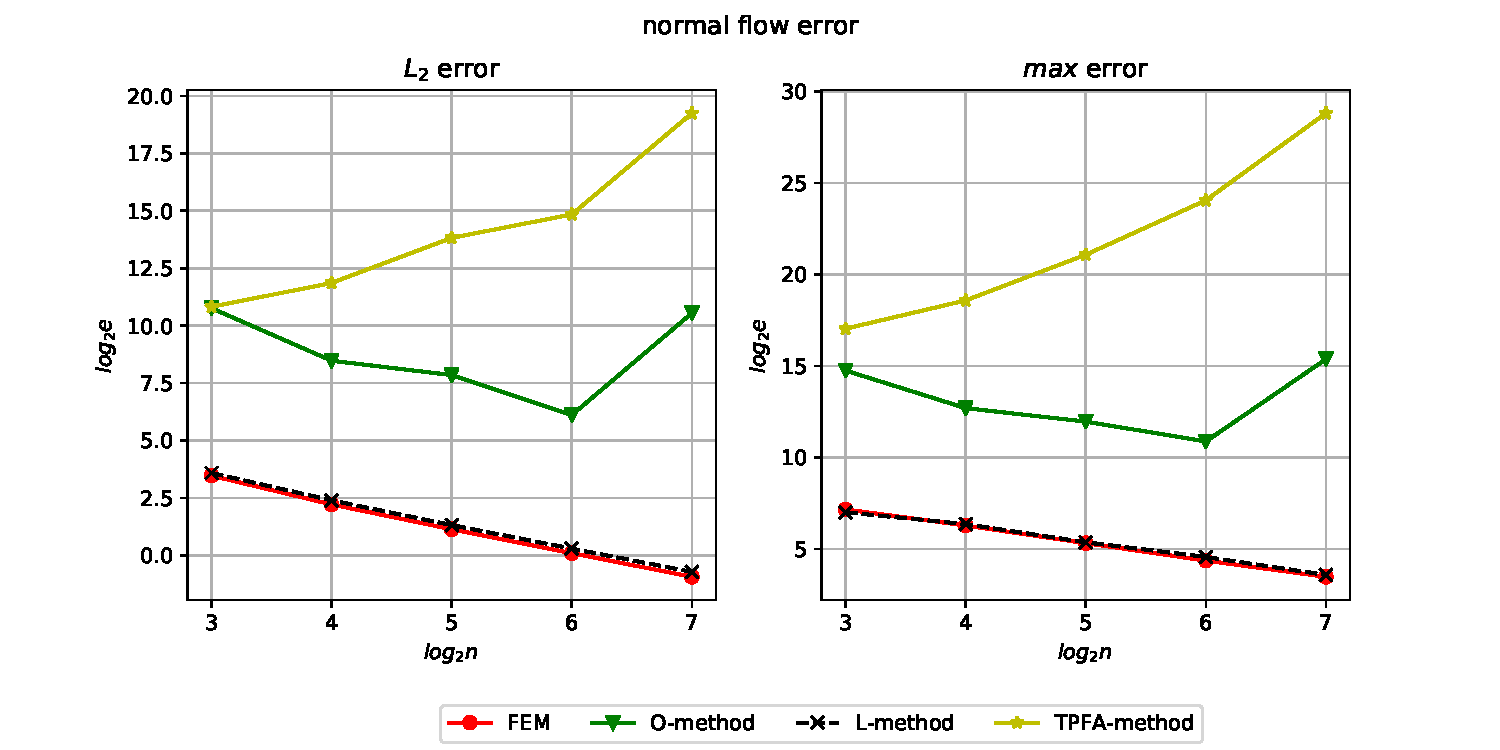
\includegraphics[width=1.2\textwidth]{flow_aspect100.pdf}
			\caption{The normal flow density error of perturbed mesh with aspect ratio 0.01.}
			\label{fig:mesh_perturbed_flow_1d100}
		\end{figure}
	\section{Richards' Equation}
	\label{sec:numerics_richards}
	\todo[inline]{This section is not yet done}
	\subsection{Constant Hydraulic Conductivity}
	In this section we consider numerical experiments for \eqref{eq:richards simple}, with Dirichlet boundary conditions: Find $u=u(x,t)$ such that
	\begin{equation}\label{eq:richards_conv_1}
			\left \{
		\begin{aligned}[c]
			\partial_t b(u) - \nabla \cdot \nabla u &= f, \\
			u &= u|_{\Gamma_D}, \\
			u &= u_0,
		\end{aligned}
		\ \ \
		\begin{aligned}[c]
			\text{ in }& \Omega \times (0,T]\\
			\text{ on }& \partial \Gamma_D \times (0,T]\\
			\text{ on }& \Omega \times \left\{t=0\right \}
		\end{aligned}
		\right.
	\end{equation}
	We define 
	\begin{equation}\label{eq:richards_conv_2}
		b(u):=\frac{1}{1-u},
	\end{equation}
	and compute the source term, $f$, such that the solution becomes
	\begin{equation}\label{eq:richards_conv_3}
		u = -tx(1-x)y(1-y)-1.
	\end{equation}
	We let $\Omega$ be the unit square perturbed by $(x,y)  \mapsto (x-0.5y,y)$.
	The L-scheme linearization has the parameters $L:=1.5$ and error tolerance $TOL=5e^{-9}$. We perform grid refinement of a parallelogram  grid, see figure \eqref{fig:MeshRichards1}. In table \ref{tab:rihcards1} we observe a quadratic convergence when the time step length is equal to the square of the grid diameter. In table \ref{tab:rihcards2} we observe a linear convergence when the time step length and the grid diameter is equal.
	\begin{figure}[H]
	\centering
	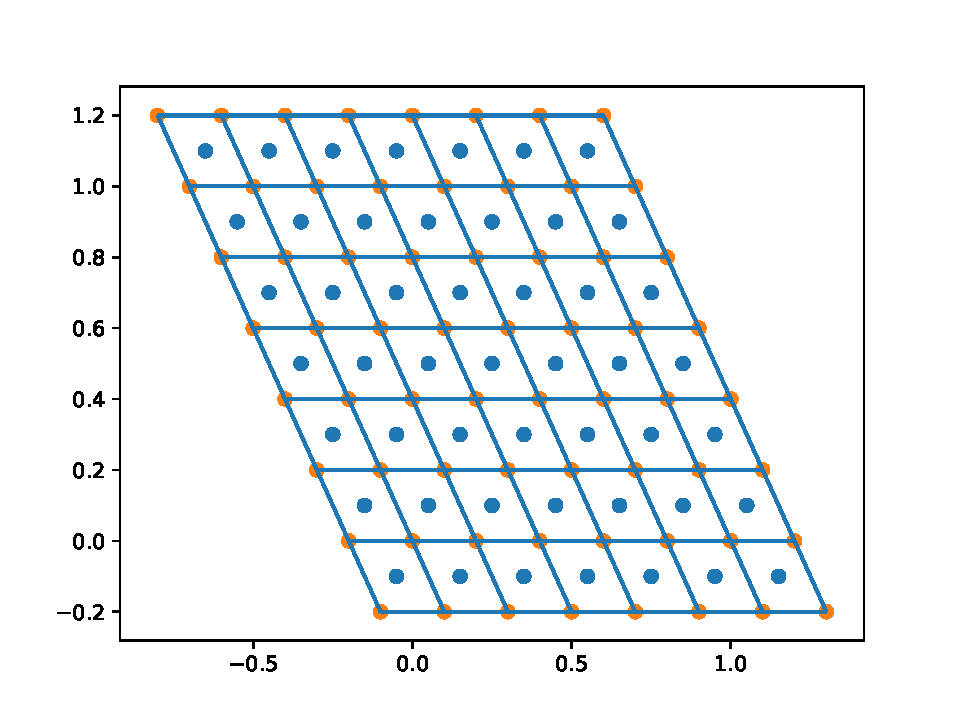
\includegraphics[width=0.8\linewidth]{MeshRichards1.pdf}
	\caption{Parallelogram grid, with ghost Dirichlet boundary cells.}
	\label{fig:MeshRichards1}
	\end{figure}
	\begin{figure}[H]
		\centering
		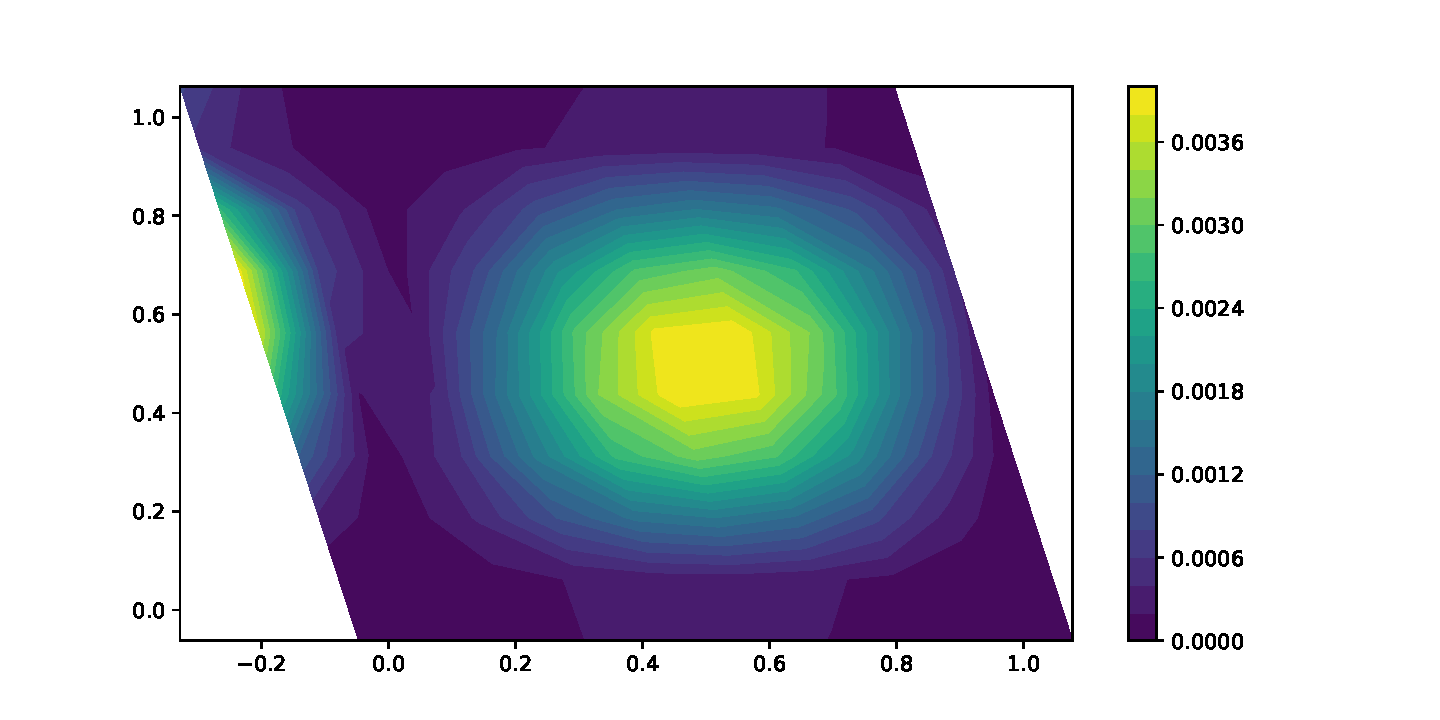
\includegraphics[width=1\linewidth]{PressureRichards11.pdf}
		\caption{The solution of \eqref{eq:richards_conv_1} at $T=1$, with the ghost Dirichlet boundary.}
		\label{fig:PressureRichards1}
	\end{figure}
	\begin{table}[H]
	\centering
	\begin{tabular}{|c c c c c|}
		\hline
			number & mesh diameter, $h$ & time step length, $\tau$ & discrete $L_2(\Omega)$ error & improvement \\
		\hline
1&$0.45069$&$0.20312$&$0.001695$&-\\ 
2&$0.22535$&$0.05078$&$0.000375$&$4.51623$\\
3&$0.11267$&$0.01270$&$0.000087$&$4.31530$\\
4&$0.05634$&$0.00317$&$0.000021$&$4.20040$\\
		\hline
	\end{tabular}
	\caption{Convergence table for \eqref{eq:richards_conv_1},\eqref{eq:richards_conv_2} and \eqref{eq:richards_conv_3}. The time step length, $\tau$, is set proportional to the square of the mesh diameter, that is $\tau=h^2$.}
	\label{tab:rihcards1}
\end{table}
	\begin{table}[H]
	\centering
		\begin{tabular}{|c c c c c|}
			\hline
			number & mesh diameter, $h$ & time step length, $\tau$ & discrete $L_2(\Omega)$ error & improvement \\
			\hline
1&$0.45069$&$0.45069$&$0.001694$&-\\ 
2&$0.22535$&$0.22535$&$0.000374$&$4.52868$\\
3&$0.11267$&$0.11267$&$0.000086$&$4.33993$\\
4&$0.05634$&$0.05634$&$0.000020$&$4.24067$\\
			\hline
		\end{tabular}
		\caption{Convergence table for \eqref{eq:richards_conv_1},\eqref{eq:richards_conv_2} and \eqref{eq:richards_conv_3}. The time step length, $\tau$, is set proportional to the square of the mesh diameter, that is $\tau=h$.}
		\label{tab:rihcards2}
	\end{table}
	\subsection{Non-Linear Hydraulic Conductivity}
	Here, we consider Richards' equation \eqref{eq:richards} in pressure variable, find $p=p(x,t)$ such that
	\begin{equation}
	\left \{
	\begin{aligned}[c]
		\partial_t \theta(p) - \nabla \cdot \kappa(\theta(p))\nabla u &= f, \\
		p &= p|_{\Gamma_D}, \\
		p &= u_0,
	\end{aligned}
	\ \ \
	\begin{aligned}[c]
		\text{ in }& \Omega \times (0,T]\\
		\text{ on }& \partial \Gamma_D \times (0,T]\\
		\text{ on }& \Omega \times \left\{t=0\right \}
	\end{aligned}
	\right.
	\end{equation}
	With $\Omega$ being the perturbed unit square as before, and $T=1$. We define 
	\begin{equation}
			\theta(u):=\left\{\begin{matrix}
				(1+(-\alpha_{vG}p)^{n_{vG}})^{-\frac{n_{vG}-1}{n_{vG}}},&p\leq 0 \\ 
				1,&p>0 
			\end{matrix}\right.
	\end{equation}
and
\begin{equation}
	\kappa(\theta):=
		\frac{\kappa_{abs}}{\mu}\sqrt{\theta}\left(1-\left(1-\theta^{\frac{n_{vG}}{n_{vG}-1}}\right)^{\frac{n_{vG}-1}{n_{vG}}}\right)^2
\end{equation}
	and compute the source term, $f$, such that the solution becomes \eqref{eq:richards_conv_3}.
	\begin{figure}
		\centering
		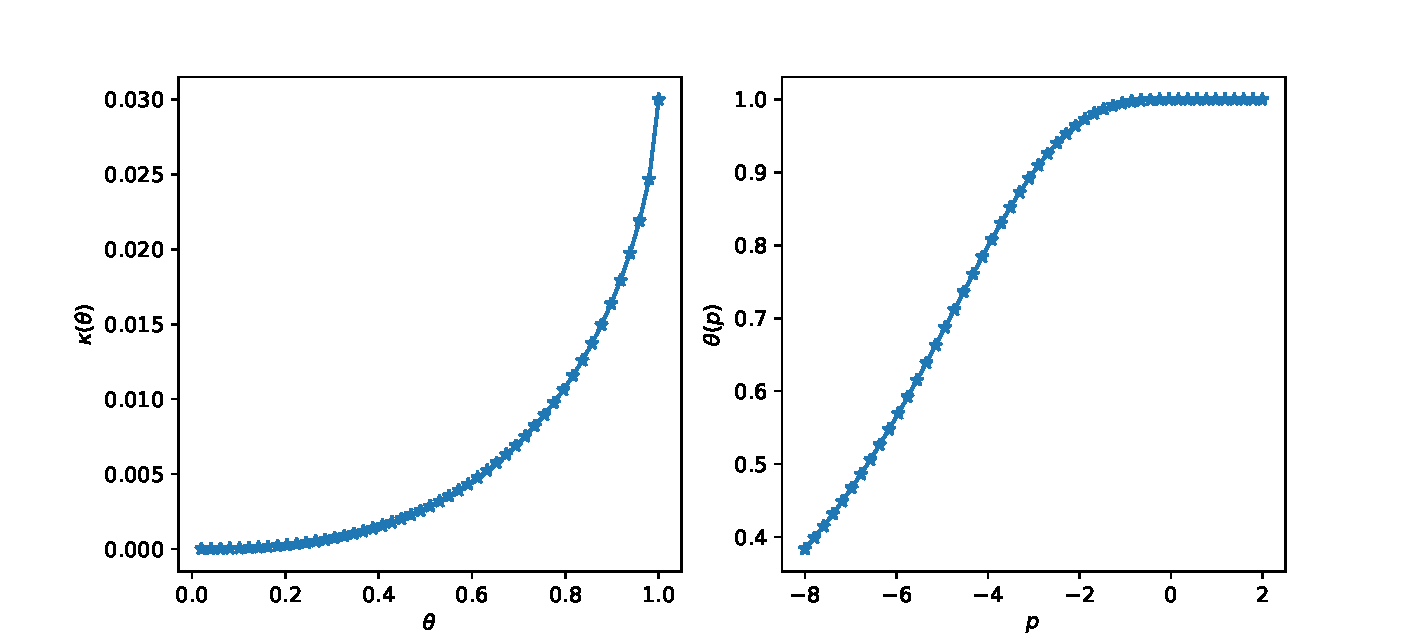
\includegraphics[width=1.1\textwidth]{van.pdf}	
	\end{figure}
	\begin{table}[H]
		\centering
		\begin{tabular}{|c c c c c|}
			\hline
			number & mesh diameter, $h$ & time step length, $\tau$ & discrete $L_2(\Omega)$ error & improvement \\
			\hline
				1&$0.45069$&$0.20312$&$0.001863$&-\\ 
				2&$0.22535$&$0.05078$&$0.000455$&$4.09403$\\ 
				3&$0.11267$&$0.01270$&$0.000110$&$4.13154$\\
			\hline
		\end{tabular}
		\caption{Convergence table for \eqref{eq:richards_conv_1},\eqref{eq:richards_conv_2} and \eqref{eq:richards_conv_3}. The time step length, $\tau$, is set proportional to the square of the mesh diameter, that is $\tau=h^2$.}
		\label{tab:rihcards1}
	\end{table}
	\begin{table}[H]
		\centering
		\begin{tabular}{|c c c c c|}
			\hline
			number & mesh diameter, $h$ & time step length, $\tau$ & discrete $L_2(\Omega)$ error & improvement \\
			\hline
1&$0.45069$&$0.45069$&$0.017904$&-\\ 
2&$0.22535$&$0.22535$&$0.006011$&$2.97848$\\
3&$0.11267$&$0.11267$&$0.001682$&$3.57467$\\
			\hline
		\end{tabular}
		\caption{Convergence table for \eqref{eq:richards_conv_1},\eqref{eq:richards_conv_2} and \eqref{eq:richards_conv_3}. The time step length, $\tau$, is set proportional to the square of the mesh diameter, that is $\tau=h$.}
	\end{table}
\end{document}